\chapter{Open-source platformy}
Tato kapitola se zaměřuje na možnost vizualizace a ovládní domácí automatizace pomocí open-source technologií (software s otevřeným kódem), které je možné využít v případě nedostatku financí nebo pro uživatele, kteří chtějí mít plnou kontrolu nad svým systémem. V případě tohoto řešení byl vybrán přístup pomocí kontejnerizace, který umožňuje snadné nasazení a škálování aplikací, ale také snadné zálohování a migraci v případě poruch.

\section{Raspberry Pi 5}
Jedná se o jednodeskový počítač, který je určen pro široké spektrum aplikací od IoT, rozpoznávání obrazu, strojového učení, robotiky až po multimediální aplikace. Mezi hlavní výhody patří nízká cena, malé provozní náklady, možná modularita přes GPIO piny, PCI expres a USB porty a velké množství tzv. HAT modulů, které jsou určeny pro rozšíření funkcí. \cite{Raspberry Pi 5}.

Pro tuto aplikaci bylo zvoleno Raspberry Pi 5 s 16 GB RAM, pamětí 256 GB a operačním systémem Raspberry Pi OS, který je stavěn na Linuxové distribuci Debianu. Hlavním důvodem výběru byla nízká cena, ale i jednoduchá dostupnost pro případného zájemce o domácí automatizaci, který by si chtěl systém ovládání a vizualizace vytvořit sám.

Jediným závažnějším problémem tohoto zařízení je degradace paměťové karty, na které je nahrán operační systém. Tento problém je způsoben častým zápisem, který postupně snižuje životnost, rychlost a velikost paměti. V krajních případech může dojít i k úplnému zničení a ztrátě dat. K předcházení tohoto problému se historicky používala technika \textit{wear leveling} - rozložení zápisu na celou paměťovou kartu, aby se snížil počet zápisů na jednotlivé buňky \cite{wear leveling}. Teď už je možné použít M.2 NVMe SSD disk, který je připojen přes PCI expres a je mnohem rychlejší než paměťová karta. Tento disk je možné použít i jako bootovací disk, což zamezí problémům s bootováním a ztrátou dat. Další možností, jak zpomalit tuto degradaci, je připojení USB flash disku. Flash disk dokáže zamezit opotřebování paměti díky přenesení souborů s vyšší frekvencí zápisu - v tomto případě databáze, nicméně rychlost zápisu se tímto sníží.
\begin{figure}[!ht]
    \begin{center}
        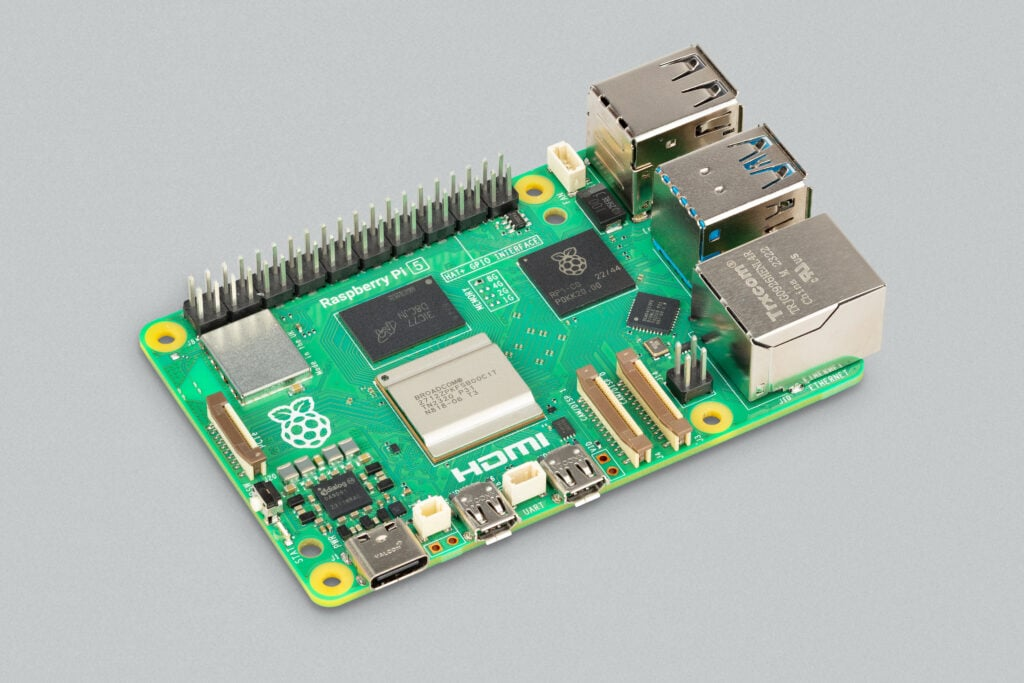
\includegraphics[scale=0.30]{obrazky/RaspberryPi5.jpg}
    \end{center}
    \caption[Raspberry Pi5~\cite{Raspberry Pi 5}]{Raspberry Pi5~\cite{Raspberry Pi 5}}
    \label{fig:RaspberryPi}
\end{figure}
\newpage
Alternativou k Raspberry Pi 5 mohou být LattePanda, ASUS NUC a podobné mikropočítače, které mají vyšší výkon, větší možnost výběru operačního systému (dostatečný výkon na Windows) a robustnost. Tyto výhody jsou kompenzovány vyšší pořizovací cenou, spotřebou a velikostí.
\section{Docker Compose}
Docker Compose je nástroj pro definici a správu více kontejnerových aplikací. Umožňuje uživatelům definovat aplikaci pomocí \textit{YAML} souboru, které obsahují informace o kontejnerových službách, sítích a úložištích. \cite{Docker Compose}

Instalace Docker Compose je jednoduchá a rozepsaná na oficiálních stránkách Dockeru. Obsahuje pouze tři kroky, které jsou již připraveny pro kopírování do terminálu. \cite{DockerInstallationForDebian}

\subsection{Kontejnerizace}
Kontejnerizace je způsob virtualizace aplikací založený na linuxové technologii LXC (Linux Containers), která umožňuje spouštět aplikace v izolovaném prostředí se zárukou jejich funkčnosti v různých systémech. Tento přístup je výhodný pro nasazení aplikací s různými závislostmi a konfiguracemi a umožňuje jejich snadné nasazení i škálování. Na rozdíl od tradičních virtuálních strojů poskytuje kontejnerizace kompletní běhové prostředí s menšími nároky na výkon a paměť, protože nevyžaduje samostatný kernel ani simulaci veškerého hardwaru. \cite{ContainerAndVirtualization}
V případě této práce byl navrhnut Docker Stack, který je složen z několika kontejnerů, které spolu komunikují a vytváří tak komplexní systém na ovládání a vizualizaci domácí automatizace. Vzhled tohoto stacku i s komunikacemi je zobrazen na Obr. \ref{fig:DockerStack}.
\begin{figure}[!ht]
    \begin{center}
        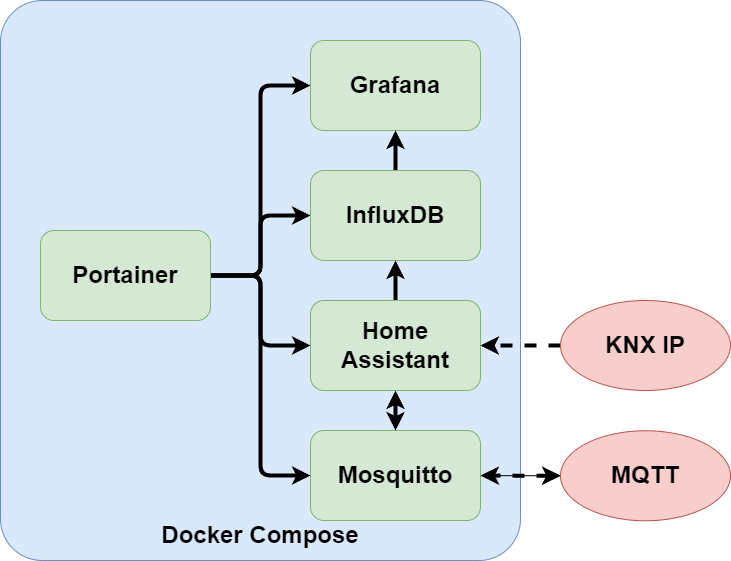
\includegraphics[scale=0.30]{obrazky/stack.png}
    \end{center}
    \caption[Docker Stack]{Docker Stack }
    \label{fig:DockerStack}
\end{figure}
\subsection{Tvorba YAML souboru}
YAML soubor je textový soubor, který obsahuje definici kontejnerů a jejich konfigurací. Je napsán v jazyce YAML (YAML Ain't Markup Language), což je formát pro serializaci dat \cite{YAML}. Níže je příklad vzhledu YAML souboru (Výpis \ref{lst:dockeryaml}), který by měl pomoci ke snadnému pochopení struktury a syntaxe \cite{ComposeYamlExample}.

Dále pak může YAML soubor obsahovat i enviromentální proměnné, které se používají k nastavení kontejneru. Tyto proměnné mohou být obsaženy v souboru .env, který se používá k uchovávání citlivých informací, jako jsou například hesla a API klíče. Tento soubor je načítán při spuštění kontejneru. \cite{ENV}
\begin{lstlisting}[language=YAML, breaklines=true, numbers=left, numberstyle=\small, numbersep=10pt, frame=single, basicstyle=\ttfamily\small, caption=YAML soubor, label=lst:dockeryaml]
version: "3" # Verze Docker Compose
services: # Sluzby
    name_of_service: # Jmeno sluzby
        image: name_of_image:latest # Jmeno image
        container_name: name_of_container # Jmeno kontejneru
        networks: # Site
            - name_of_network # Jmeno site na ktere pobezi kontejner
        depends_on: # Zavislosti
            - name_of_service # Jmeno kontejneru na kterem zavisi
\end{lstlisting}
\pagebreak
\begin{lstlisting}[language=YAML, breaklines=true, numbers=left, firstnumber=10, numberstyle=\small, numbersep=10pt, frame=single, basicstyle=\ttfamily\small]
        environment: # Promenne prostredi
            - PUID=1000 # ID uzivatele, ktery bude mit pristup k souborum
            - PGID=1000 # ID skupiny, ktera bude mit pristup k souborum
            - TZ=Europe/Prague # Casove pasmo
            - WEBUI_PORT=1234 # Port na kterem pobezi webove rozhrani 
            - DOCKER_MODS="linuxserver/mods:universal" # Docker modifikace
        volumes: # Slozky, ktere budou pripojeny do kontejneru
            - "/path/on/host:/path/in/container" # Cesta k souborum
        ports: # Porty pro pripojeni k hostitelske site
            - "host_port:container_port"
        deploy: # Nasazeni kontejneru
            resources:
                limits:
                    memory: 512m # Maximalni pamet
                    cpus: "1" # Maximalni CPU
                reservations:
                    memory: 256m # Minimalni pamet
                    cpus: "0.5" # Minimalni CPU
        restart: always # Restart kontejneru pri padu
        labels: # Metada
            - "com.docker.compose.project=project_name" # Nazev projektu
            - "com.docker.compose.service=service_name" # Nazev sluzby
            - "com.docker.compose.version=1.0" # Verze sluzby
\end{lstlisting}
\noindent Celková implementace a je zobrazena v příloze~\ref{apend:dockeryaml}.
\subsection{Portainer}
Jedná se o open-source kontejner, který slouží jako webové rozhraní pro správu Dockeru. Umožňuje uživatelům spravovat kontejnery, image (obrazy – šablony pro vytváření kontejnerů), 
stohy (stohy – skupiny kontejnerů, které spolu komunikují), sítě, uložiště, čtení logů, sledování výkonu, správa portů a další funkce. Jednou z předních výhod je jednoduchost použití; kromě rozhraní (Obr.~\ref{fig:portainer}) je i propojení s Docker Hubem, což je veřejná knihovna kontejnerů. \cite{Portainer} 
\begin{figure}[!ht]
  \begin{center}
  \includegraphics[scale=0.39]{obrazky/portainer.png}
  \end{center}
  \caption[Portainer Stack]{Portainer Stack}
  \label{fig:portainer}
\end{figure}
\pagebreak
\section{Mosquitto}
Mosquitto je open-source broker společnosti Eclipse pro protokol MQTT (Message Queuing Telemetry Transport – více v podkapitole \ref{subsection:MQTT}). Zajišťuje komunikaci mezi vydavatelem a odběratelem v závislosti na oprávněních a kvalitě služeb (\textit{QoS}). Jednou z výhod tohoto brokeru je jednoduchost implementace a nízké nároky na výkon. Dále umožňuje šifrování pomocí \textit{TLS}, které zajišťuje bezpečnost přenosu dat, podporuje cloudové služby a různé platformy. K dispozici je také knihovna pro jazyk \textit{C}, která implementuje celý protokol. \cite{Mosquitto}

V této práci byl použit kontejner pro komunikaci mezi Home Assistantem a PLC. Tento kontejner byl nastaven na porty 1883 a 9001. Port 1883 je standardní port pro MQTT protokol a používá se ke komunikaci mezi brokerem a PLC. Port 9001 je určen pro WebSocket, což je protokol pro komunikaci mezi webovými aplikacemi a servery. Proto byl použit pro komunikaci mezi Home Assistantem a Mosquittem.

Různé porty v brokeru nemají vliv na funkčnost komunikace, protože broker je schopen komunikovat na více portech současně. To znamená, že broker může přijímat zprávy na jednom portu a odesílat je skrze jiný port, pokud je použito správné téma (\textit{topic}). Dále nezáleží na pořadí příchodu zpráv, protože broker je zpracovává sekvenčně – v pořadí, v jakém přišly.
\section{Home Assistant}
Home Assistant je open-source platforma pro domácí automatizaci, která v posledních letech získala velkou popularitu. Umožňuje propojení více zařízení různých výrobců, databází a protokolů do jednoho systému. Dále pak umožňuje uživatelům monitorovat spotřebu, vytvářet vlastní vizualizace, automatizace a scénáře pro ovládání zařízení. Tato platforma je dostupná v kontejnerové podobě, jako operační systém nebo jako virtuální stroj. \cite{Home Assistant}

Jednotlivá zařízení lze implementovat prostřednictvím tzv. integrací, které jsou buď předinstalované v Home Assistantu, nebo dostupné jako pluginy. Portfolio zařízení i funkcí lze dále rozšířit pomocí komponent vyvíjených komunitou, které jsou dostupné prostřednictvím pluginu \textit{HACS} (Home Assistant Community Store). \cite{HACS}

Přidání KNX zařízení do Home Assistantu je možné pomocí integrace \textit{KNX}, která umožňuje implementaci skrze YAML soubor, ale také pomocí webového rozhraní. V této práci byla zvolena druhá možnost, která je jednodušší a rychlejší. Prvním krokem byl výběr a nastavení spojení s KNX - \textit{routing}, \textbf{\textit{tunneling}} (více v podkapitole \ref{KNXnet/IP}). Dalším krokem bylo vložení projektu instalace vygenerovaného pomocí \textit{ETS}, který obsahoval všechny potřebné informace o zařízeních a jejich adresách. Posledním krokem byla tvorba jednotlivých entit, které se vkládaly pomocí webového rozhraní - výběr typu entity, její název a adres jednotlivých funkcí. Například pro světlo bylo potřeba nastavit adresu pro ovládání, adresu pro stav, adresu pro jas a adresy pro nastavení barev. Tyto adresy se pak vybíraly ze seznamu, který se vygeneroval při vložení projektu. Existuje také možnost použít i vlastní adresy, které v projektu dosud neexistují.

Pro komunikaci mezi Home Assistantem a PLC byla použita integrace \textit{MQTT}, která se nastavila pomocí webového rozhraní a konfiguračního souboru YAML (Příloha \ref{apend:configyaml}). Webové rozhraní slouží k nastavení IP adresy, portu, uživatelského jména a hesla pro připojení k brokeru. YAML soubor slouží pro vytvoření jednotlivých entit.

Po vytvoření všech entit jim byl přidělen název, ikona a byly rozděleny do různých skupin podle místa použití (záložka \textit{Area}). Důsledkem tohoto kroku byla automaticky vygenerována vizualizace, která sloužila k hrubému ovládání a sledování stavu jednotlivých zařízení (Obr. \ref{fig:HAvisu1}).

\begin{figure}[!ht]
    \begin{center}
        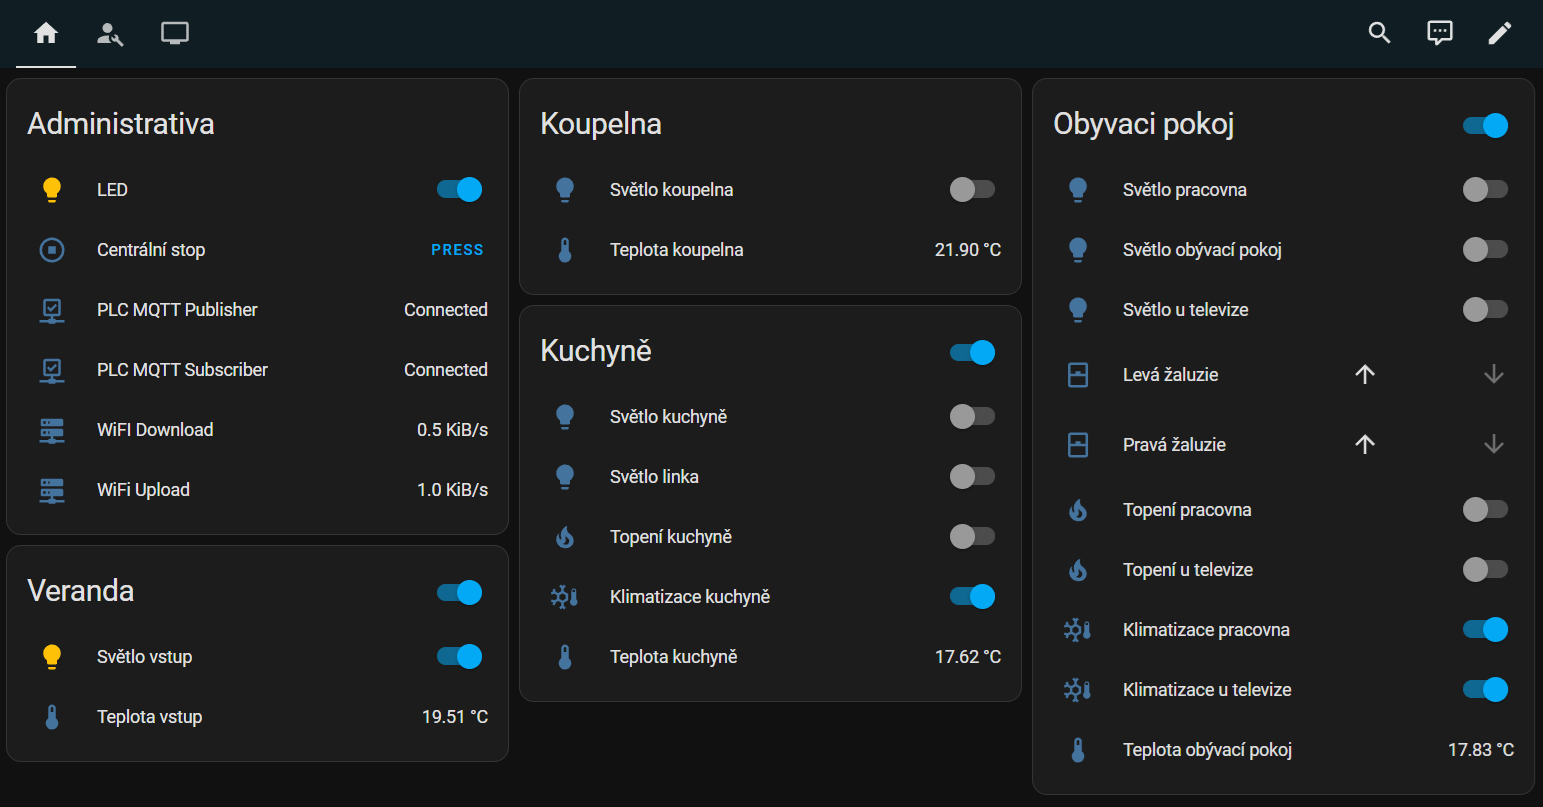
\includegraphics[scale=0.35]{obrazky/Dashboard1.png}
    \end{center}
    \caption[Home Assistant hrubá vizualizace]{Home Assistant hrubá vizualizace}
    \label{fig:HAvisu1}
\end{figure}

Pro jednodušší ovládání a přehlednost byly vytvořeny vlastní vizualizace. První byla vytvořena podle skupin ovládaných prvků (Obr. \ref{fig:HAvisu2}), druhá byla vytvořena podle místností (Obr. \ref{fig:HAvisu3}). Dále na nich byly použity jiné možné vzhledy jednotlivých prvků, které nabízí základní verze Home Assistantu. Pro případ, že by se ani ty uživateli nelíbily, je možné otevřít vyskakovací okna jednotlivých prvků, které nabízí více možností ovládání. V těchto oknech lze také sledovat historii jednotlivých prvků.

\begin{figure}[!ht]
    \begin{center}
        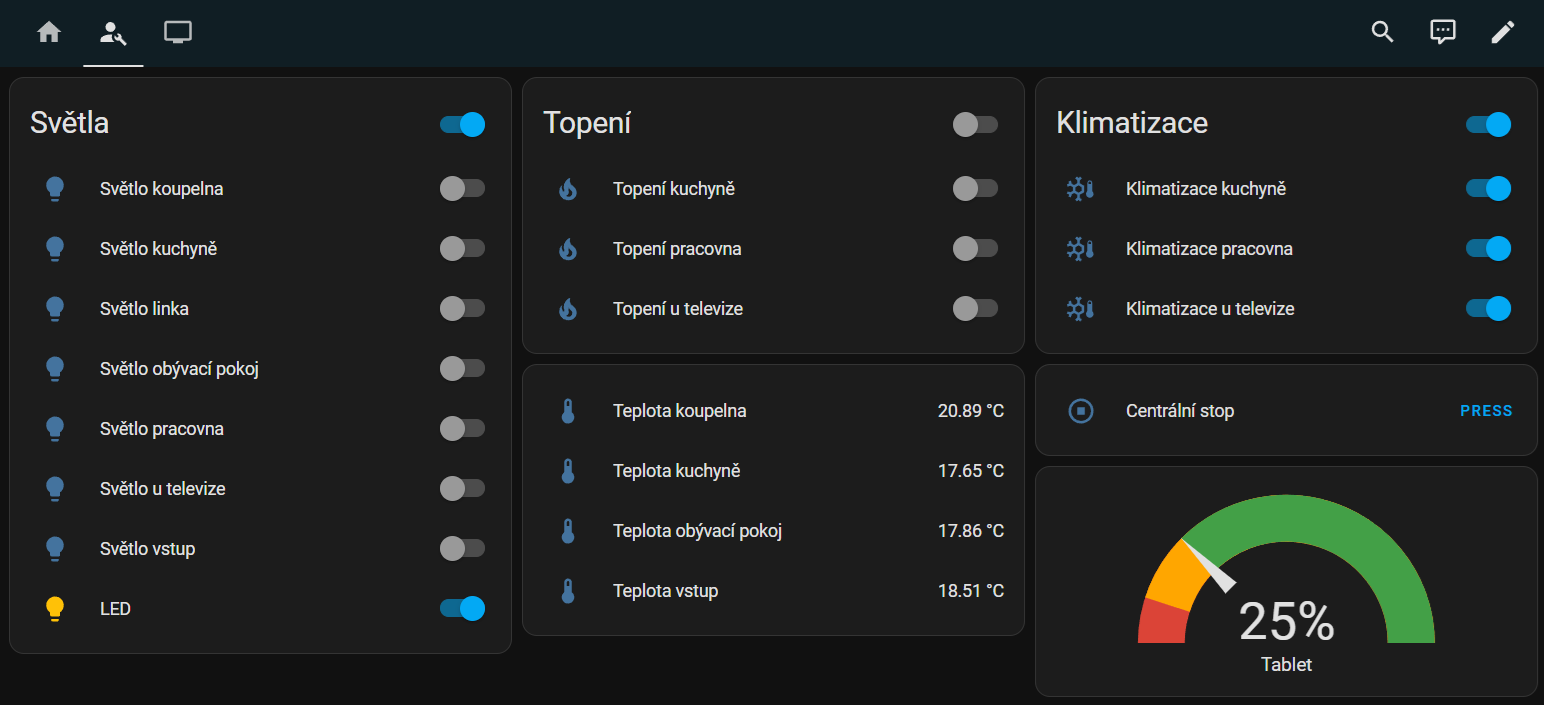
\includegraphics[scale=0.35]{obrazky/Dashboard2.png}
    \end{center}
    \caption[Home Assistant funkční vizualizace]{Home Assistant funkční vizualizace}
    \label{fig:HAvisu2}
\end{figure}

\begin{figure}[!ht]
    \begin{center}
        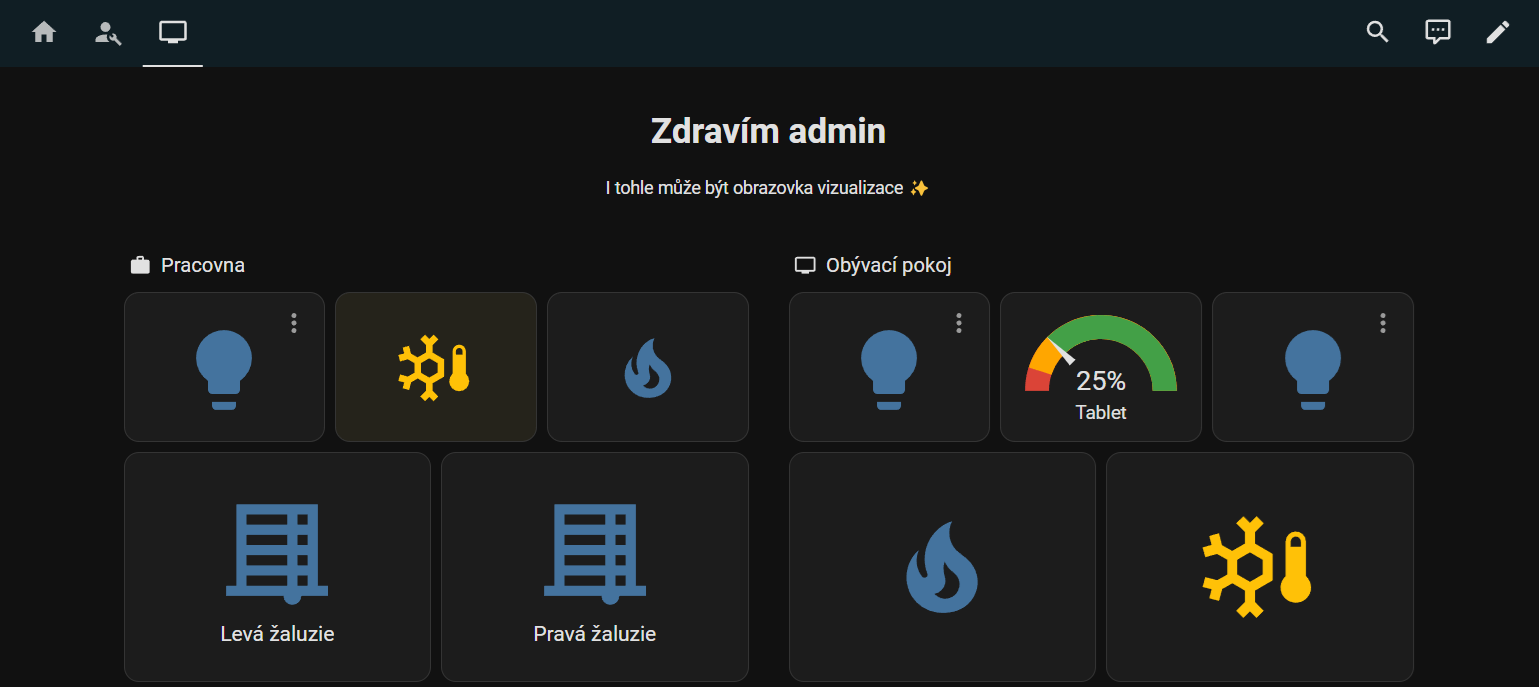
\includegraphics[scale=0.35]{obrazky/Dashboard3.png}
    \end{center}
    \caption[Home Assistant vizualizace dle umístění]{Home Assistant vizualizace dle umístění}
    \label{fig:HAvisu3}
\end{figure}

Pro potřebu sledování historie jednotlivých zařízení je možné použít vestavěnou funkci Home Assistantu - \textit{History}, která zobrazuje blízkou historii. Pro sledování delší historie bohužel neexistuje adekvátní řešení, protože Home Assistant ukládá historii do SQLite databáze, která není určena pro dlouhodobé ukládání dat. Proto byla použita integrace \textit{InfluxDB}. Další výhodou použití externí databáze je možnost sledovat historii i bez připojení k Home Assistantu. 

Připojení této databáze je uvedeno v příloze~\ref{apend:configyaml}.
\section{InfluxDB}
Jedná se o open-source databázi určenou pro ukládání časových řad. Databáze je optimalizována pro čtení a zápis velkého množství dat, která se následně využívají k analýze v reálném čase. Její hlavní výhodou je rychlost a efektivita při práci s velkým množstvím dat. Pro udržení rychlosti byly implementovány retenční politiky, které určují, jak dlouho se data uchovávají a jakým způsobem se agregují. \cite{InfluxDB} \newline

Databáze je tvořena několika základními koncepty~\cite{InfluxDBKeyConcepts}:
\begin{itemize}
    \item \textbf{Bucket} – kontejner pro ukládání dat
    \item \textbf{Measurement} – popis dat ukládaných do bucketu
    \item \textbf{Series} – skupina bodů se stejným tagem a měřením
    \item \textbf{Point} – jednotkový záznam v bucketu
    \item \textbf{Field} – hodnota ukládaná do bucketu
    \item \textbf{Tag} – klíč používaný k identifikaci dat v bucketu
    \item \textbf{Timestamp} – časový údaj o uložení dat
    \item \textbf{Retention policy} – pravidlo pro uchovávání dat v bucketu
    \item \textbf{Continuous query} – dotaz, který se provádí automaticky v pravidelných intervalech.
\end{itemize}
Kontejner této databáze běží na portu 8086. Po vytvoření kontejneru je potřeba nastavit uživatelské jméno a heslo pro přístup do databáze. Dále je potřeba nastavit bucket, do kterého se budou ukládat data – základní informace, délku uchovávání, způsob agregace dat a přístup přes API. Všechny tyto informace se nastavují pomocí webového rozhraní.

Webové rozhraní také umožňuje vytvářet a spravovat uživatelské účty a přístupová práva, sledovat výkon databáze, historii jednotlivých dat a vytvářet pro ně dotazy, které se provádějí pomocí jazyka \textit{Flux}. Tyto dotazy slouží k analýze dat a vytváření grafů, a to buď přímo v InfluxDB, nebo pomocí externích nástrojů, jako je Grafana. 
\section{Grafana}
Grafana je open-source platforma pro vizualizaci a analýzu dat. Umožňuje uživatelům vytvářet interaktivní grafy, tabulky a panely pro zpracování dat z různých zdrojů a také nastavovat upozornění na základě těchto dat. Disponuje širokým portfoliem pluginů, které umožňují připojení k různým databázím a službám. Grafana je velmi populární mezi vývojáři a administrátory, kteří potřebují monitorovat a analyzovat data v reálném čase. \cite{Grafana} \newline

Vizualizace v Grafaně je tvořena pomocí přehledů (dashboardů), které obsahují panely. Tyto panely mohou mít různé typy grafů~\cite{GrafanaVisualization}:
\begin{itemize}
    \item \textbf{Grafy a diagramy}
    \begin{itemize}
        \item \textbf{Time series} – data v čase
        \item \textbf{State timeline} – stav v čase
        \item \textbf{Status history} – periodický stav v čase
        \item \textbf{Bar chart} – kategoriální data
        \item \textbf{Histogram} – rozložení dat prezentované jako sloupcový graf
        \item \textbf{Heatmap} – vizualizace dat ve dvou rozměrech, typicky velikosti jevu
        \item \textbf{Pie chart} – zobrazení proporcionality
        \item \textbf{Candlestick} – typicky pro finanční data
        \item \textbf{Gauge} – zaoblený ukazatel zobrazující, jak daleko je metrika od prahu
        \item \textbf{Trend} – datové sady se sekvenčním, číselným x, které není čas
        \item \textbf{XY chart} – vizualizace hodnot x a y v grafu
    \end{itemize}
    \item \textbf{Statistika a čísla}
    \begin{itemize}
        \item \textbf{Stat} – velké statistiky a změny v čase
        \item \textbf{Bar gauge} – horizontální nebo vertikální ukazatel
    \end{itemize}
    \item \textbf{Různé}
    \begin{itemize}
        \item \textbf{Table} – vizualizace dat v tabulce
        \item \textbf{Logs} – vizualizace pro protokoly
        \item \textbf{Node graph} – orientované grafy nebo sítě
        \item \textbf{Traces} – trasování
        \item \textbf{Flame graph} – profilování
        \item \textbf{Canvas} – explicitní umístění prvků do statických a dynamických rozvržení
        \item \textbf{Geomap} – geoprostorová data
        \item \textbf{Datagrid} – vytváření a manipulace s daty (slouží jako zdroj dat pro jiné panely)
    \end{itemize}
    \item \textbf{Widgety}
    \begin{itemize}
        \item \textbf{Dashboard list} – seznam přehledů
        \item \textbf{Alert list} – seznam upozornění
        \item \textbf{Annotations list} – seznam anotací
        \item \textbf{Text} – markdown a HTML
        \item \textbf{News} – RSS kanály \newline
    \end{itemize}
\end{itemize}
Stejně jako v předchozích podkapitolách je i zde možné vytvářet a spravovat uživatelské účty a přístupová práva prostřednictvím webového rozhraní, tentokrát na portu 3000. \newline

\noindent Grafana v této práci sloužila jako nástroj pro zpracování historických dat instalace, konkrétně pro sledování spotřeby energie, jejího rozložení, měsíčních nákladů a historie sepnutí jednotlivých zařízení. Implementace a vzhled jednotlivých grafů jsou uvedeny v příloze \ref{apend:grafana}. 